\documentclass[tikz,border=4pt]{standalone}
\usepackage{tikz}
\usetikzlibrary{arrows.meta}
\definecolor{nebula}{HTML}{6366F1}
\definecolor{spark}{HTML}{14B8A6}
\begin{document}
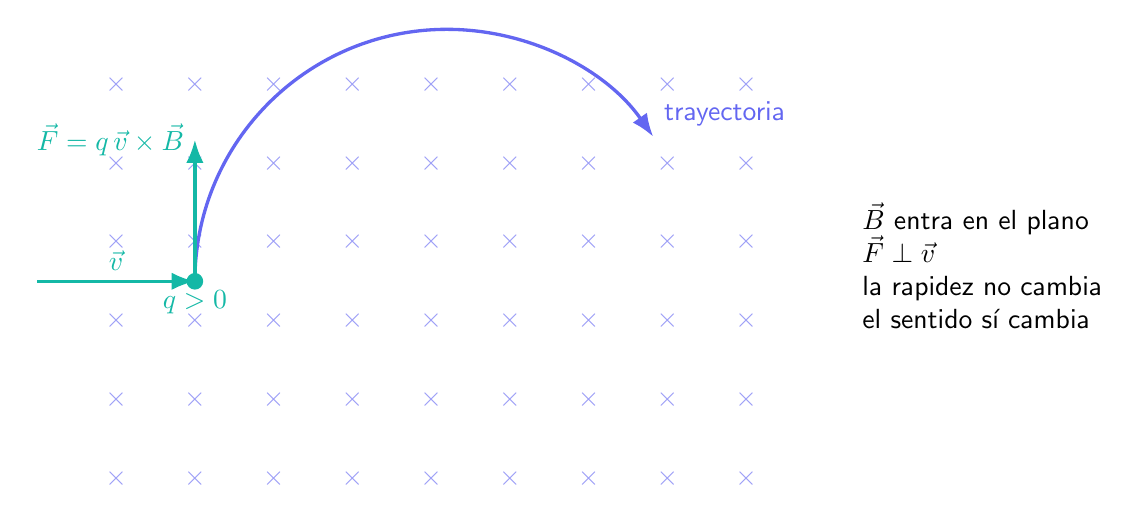
\begin{tikzpicture}[font=\sffamily,>=Latex]
  \foreach \x in {0,1,...,8}\foreach \y in {0,1,...,5}{\node[nebula!65] at (\x,\y) {$\times$};}
  \draw[->,very thick,spark] (-1,2.5)--(1,2.5) node[midway,above] {$\vec v$};
  \draw[->,very thick,nebula] (1,2.5) arc (180:35:3.2) node[above right] {trayectoria};
  \fill[spark] (1,2.5) circle(3pt) node[below] {$q>0$};
  \draw[->,very thick,spark] (1,2.5)--(1,4.3) node[left] {$\vec F=q\,\vec v\times\vec B$};
  \node[align=left,fill=white,rounded corners=3pt] at (11,2.7) {$\vec B$ entra en el plano\\$\vec F\perp\vec v$\\la rapidez no cambia\\el sentido s\'i cambia};
\end{tikzpicture}
\end{document}
